\documentclass[border=5mm, tikz]{standalone}
\usepackage{physics}
\begin{document}
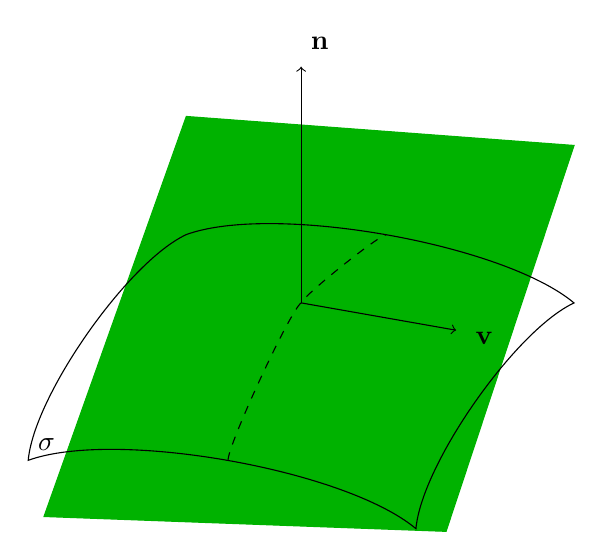
\begin{tikzpicture}[x={(170:1cm)}, y={(55:.7cm)}, z={(90:1cm)}]
    % plano
    \draw [fill, color=green!70!black] (2.5, -2, -2) -- (2.5, 2.5, 0.5) -- (-2.5, 2.5, 1) -- (-3.5, -4, 0) -- cycle;

    % superficie
    \draw[looseness=.6] (2.5,-2.5,-1) node[above right] {$\sigma$}
    to[bend left] (2.5,2.5,-1)
    to[bend left] coordinate (mp) (-2.5,2.5,-1)
    to[bend right] (-2.5,-2.5,-1)
    to[bend right] coordinate (mm) (2.5,-2.5,-1)
    -- cycle;

    \draw[dashed,looseness=.2] (mm) to[bend left] (0,0,0) to[bend left] (mp);
    
    \draw[->] (0,0,0) -- (-2,0,0) node[left, pos=1.3] {$\vb{v}$};
    % \draw[->] (0,0,0) -- (0,3,0) node[above right] {$\vb{x_{v}}$};
    \draw[->] (0,0,0) -- (0,0,3) node[right, pos=1.1] {$\vb{n}$};
    
    %\draw[dotted] (0,0,2) -- (1,0,2) -- (1,0,0);
%   \draw[->] (0,0,0) -- coordinate[pos=.3] (psi) (1,0,2) node[above left] {$\ddot{\gamma}$};
%   \node[left] at (0,0,1.5) {$\kappa_n$};
%   \node[above] at (.5,0,0) {$\kappa_g$};
%   \draw (0,0,.8) to[out=170,in=55] node[above,fill=white,inner sep=1pt,outer sep=2pt] {$\psi$} (psi);
\end{tikzpicture}
\end{document}